\subsection{Radial velocity method for exoplanet detection}
The radial velocity method is one of the few current methods of detecting exoplanets. Two celestial bodies in orbit around each other, such as a star and a planet, orbit their common center of mass (barycenter). This means that the star, although typically much more massive than the planet, is also in movement relative to an outside observer. The larger the planet is, compared to the star, the larger this movement will be. For now, it is not possible to directly observe exoplanets. One way of indirect detection however is thus measuring the movement of the star. We can measure the relative movement of a star through the doppler effect; the electromagnetic spectrum of the star observed on Earth will be blue shifted when the star is moving toward us and red shifted when moving away. The potential indirect signal of a planet will thus consist of a periodic doppler shift in the spectrum of the host star. For this method in general, several years of data collection is necessary. One should at least have one full orbit of observational data, and, to decrease statistical uncertainties, several orbits is preferential.

A large planet like Jupiter induces a radial velocity (RV) in the Sun of about 12.7 m/s when observed in its plane of orbit. While a small one like Earth only induces an RV of about 9 cm/s. (p. 29, \cite{radial_velocity_techniques}). 

\vspace{0.5cm}
\todo{Possibly describe the RV calculation in more \href{http://exoplanets.astro.yale.edu/workshop/EPRV/Bibliography_files/Radial_Velocity.pdf}{detail} and compute Earth K. } 

\subsubsection{Doppler shift}

The radial velocity method relies on the well-known Doppler effect. Ignoring terms of $c^-4$ and higher, the general shift caused by a relative displacement betweeen the source and an observer at zero gravitatonal potential is given by 

\begin{equation}
    \label{eq:doppler_GR_SR}
    \lambda=\lambda_{0} \frac{1+\frac{1}{c} \mathbf{k} \cdot \mathbf{v}}{1-\frac{\Phi}{c^{2}}-\frac{v^{2}}{2 c^{2}}},
\end{equation}

which accounts for both special relativistic effects and gravitatonal doppler shift described by general relativity. Where $\lambda$ is the observed wavelength, $\lambda_0$ is the emitted wavelength, $\Phi$ is the Newtonian gravitational potential at the source $(\Phi=G M / r$ at a distance $r$ of a spherically symmetric mass $M$ ), $\textbf{k}$ is the unit vector pointing from the observer to the source, $\textbf{v}$ is the velocity of the source relative to the observer and $c$ is the speed of light \cite{doppler_shift_GR_formula}.

Special relativistic effects we can safely ignore, as we are dealing with velocity shifts on the order of meters or centimeters per second, and thereby cross out the third term in the denominator. The remaining terms $(1-\Phi/c^2)$ evaluted for HD 34411 ($M = (1.08 \pm 0.14) M_{\odot}$, $R = (1.28 \pm 0.04) R_{\odot}$ \cite{star_properties}) is around $0.999998$. \todo{}I don't quite know how to check analytically if this will have an influence on the errors on A given by imniuit. Running the program it doesn't... So, we can neglect the denominator completely.

If the unit vector $\textbf{k}$ were pointing directly toward us, it would mean that we were observing the system in the plane of orbit. This is however unlikely. Since we don't know the inclication angle, a possible simplification is to omit $\textbf{k}$ is treat the resulting $\textbf{v}$ as a minimum radial velocity.

Thus we are left with 

\begin{equation}
    \label{eq:our_doppler}
    \lambda = \lambda_0 \times \Big(1 + \frac{v}{c} \Big),
\end{equation}

which is to say that the observed wavelength is simply the emitted wavelength scaled by a factor $(1 + v/c)$. This formula allows us to compute the minimum relative velocity shift, $v$, between two observations, $\lambda$ and $\lambda_0$.


\subsection{Description of the instrument}
The EXtreme PREcision Spectrograph or EXPRES is an extreme-precision spectrograph situated at the Lowell Observatory's 4.3m Lowell Discovery Telescope (LDT) near Flagstaff, Arizona, USA. The LDT allows for up to 280 partial nights of observation per year.

Like in many spectrographs, at the heart of EXPRES is a Charge Coupled Device (CCD). A CCD is a silicon-based multi-channel photon detector consisting of a large number of small light-sensitive areas called pixels. The CCD is EXPRES an STA1600LN CCD backside illuminated image sensor with a $10,560 \times 10,560$ array containing 9µm$\times$9µm pixels, designed to with a wavelength range of 3800$-$7800Å. When a photon hits a pixel it is converted into a charge, and each pixel can thus supply independent measurements. Since a one dimensional sensor would be impractical, EXPRES is constructed in such a way, that it wrap the spectrum inside the CDD, meaning that the spectrum starts in the top row of the sensor, and continues in the second row. Short wavelengths are thus to be found in the top of the CCD and long wavelengths at the bottom.

EXPRES has a spectral resolution of $R = 150'000$, where R is defined as $R = \lambda / \Delta\lambda$, such that, say at a wavelength of $\lambda = 5000$Å, EXPRES should be able to detect a wavelength shift of $\Delta\lambda = 5000\text{Å}/150'000 \approx 0.033 $Å. \todo{Add m/s}. 

EXPRES is housed in a vacuum enclosure to minimize changes in temperature and pressure, which can otherwise cause the spectra to change position on the CCD and thus lead to errors in the RV mesaurements. 

Wavelength calibrations are performed with the use of a Laser Frequency Comb 
(LFC), produced by Menlo Systems, which is a laser source whose spectrum consists of a series of discrete, equally spaced frequency lines. The LFC however also needs calibration for which a Thorium Argon (ThAr) lamp with known frequencies is used.

Barycentric corrections are derived from the EXPRES exposure-meter, which is essentially a smaller, less precise spectrograph. Described in detail in \cite{barycentric_exposure_meter_blackman}. EXPRES as a whole is described in technical detail in \cite{EXPRES_technical_details_Jurgenson}.


\subsection{Description of the data}
EXPRES data are meant to serve as an example of the data being produced by next-generation spectrographs. 

The data used in this project was supplied by Lily Zhao and is by no means raw data, but data that has already gone through a lot of processing.

For development of RV extraction method, observations from four stars were used: 

\begin{itemize}
    \item HD 101501 (45 observations, 22 nights, Feb. 10, 2019 - Nov. 26, 2020)
    \item HD 26965 (114 observations, 37 nights, Aug. 20, 2019 - Nov. 27, 2020)
    \item HD 10700 (174 observations, 34 nights, Aug. 15, 2019 - Nov. 27, 2020)
    \item HD 34411 (188 observations, 58 nights, Oct. 08, 2019 - Nov. 27, 2020)
\end{itemize}

The observations for HD34411 are plotted in figure \ref{fig:dates_HD34411}. Most days have 3-4 observations, and there are significant gaps in the data as well.

\begin{SCfigure}[1][!h]%
    \begin{wide}  
        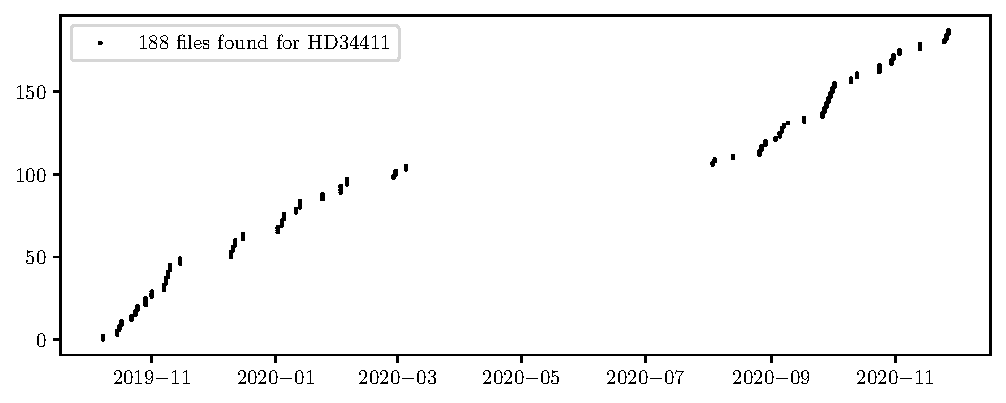
\includegraphics[width=\textwidth]{figures/dates_HD34411.pdf}
        \caption{EXPRES observations of HD 34411}
    \label{fig:dates_HD34411}
    \end{wide}
\end{SCfigure}
        
\todo{Specify which data was used for LFC calibration method development}

\subsubsection{Data structure}
The data used in this project consists of already packaged FITS (Flexible Image Transport System) files, which is a portable file standard widely used in the astronomy community to store images and tables. There is a FITS file for each observation, containing a variety of mesaurements for each pixel on the CCD. 
The rows of the CCD data are referred to as orders. There are 86 orders each of which has values from 7920 pixels. Drawing a coordinate system on the CCD, we are thus moving through pixels as we go along the x-axis and through orders as we go along the y-axis.

This would give the CCD the very elonganted dimensions of 86$\times$7920, but as mentioned earlier, the CCD is actually square. The orders however hit the CCD at an angle and for this reason \emph{order tracing} is necessary. Order tracing reduces each order from 2d array to a 1d array, which means the final image comes out much shorter in the vertical/order dimension. Described in detail in section 3.2.1 of \cite{first_RV_from_EXPRES}.

Furthermore, the CCD is not equally sensitive everywhere, and there are areas along the edges that are deemed useless. The data comes with a mask which shows which pixels are should be used. 

To perform the calibration the following variables are used: \verb|spectrum|, \verb|uncertainty|, \verb|wavelength| and \verb|continuum|. To perform the RV extraction on the pre-calibrated data the following variables are used: \verb|bary_excalbur|, 
\verb|excalibur_mask|, \verb|spectrum|, \verb|uncertainty| and \verb|continuum|.

\subsubsection{Noise}
Photon noise and read noise are the two largest contributors to the noise on a given pixel on the EXPRES CCD. These two quantities are measured and summed in quadrature for each pixel. Photon noise is assumed to be poisson distributed and the standard deviation is then the square root of photon counts. Read noise is calculated emperically, details of which will not be discussed, but is assumed to be consistent throughout each night of observation. 

\subsubsection{Correction: Scatter / blaze}
Although manufactures have tried their best to limit it, the CCD still gets hits by scattering light, being the strongest in the center of the detector. It is modeled and subtracted by measureing the photon count in between orders.

\subsubsection{Correction: Tellurics}
Tellurics (general definition being originating from the Earth) in this context refers to the contamination that ground based spectrographs have to deal with, which occurs as the light passes through the Earth's atmosphere, encountering molecules such as oxygen and water vapor. On EXPRES the technique used is called SELENITE [https://arxiv.org/pdf/1903.08350.pdf].

\subsubsection{Correction: Barycentric corrections}
\todo{}




